%%%%%%%%%%%%%%%%%%%%%%%%%%%%%%%%%%%%%%%%
% Arsclassica Article
% LaTeX Template
% Version 1.1 (10/6/14)
%
% This template has been downloaded from:
% http://www.LaTeXTemplates.com
%
% Original author:
% Lorenzo Pantieri (http://www.lorenzopantieri.net) with extensive modifications by:
% Vel (vel@latextemplates.com)
%
% License:
% CC BY-NC-SA 3.0 (http://creativecommons.org/licenses/by-nc-sa/3.0/)
%
%%%%%%%%%%%%%%%%%%%%%%%%%%%%%%%%%%%%%%%%%

%----------------------------------------------------------------------------------------
%	PACKAGES AND OTHER DOCUMENT CONFIGURATIONS
%----------------------------------------------------------------------------------------

\documentclass[
11pt, % Main document font size
a4paper, % Paper type, use 'letterpaper' for US Letter paper
oneside, % One page layout (no page indentation)
%twoside, % Two page layout (page indentation for binding and different headers)
headinclude,footinclude, % Extra spacing for the header and footer
BCOR5mm, % Binding correction
]{scrartcl}
%%%%%%%%%%%%%%%%%%%%%%%%%%%%%%%%%%%%%%%%%
% Arsclassica Article
% Structure Specification File
%
% This file has been downloaded from:
% http://www.LaTeXTemplates.com
%
% Original author:
% Lorenzo Pantieri (http://www.lorenzopantieri.net) with extensive modifications by:
% Vel (vel@latextemplates.com)
%
% License:
% CC BY-NC-SA 3.0 (http://creativecommons.org/licenses/by-nc-sa/3.0/)
%
%%%%%%%%%%%%%%%%%%%%%%%%%%%%%%%%%%%%%%%%%

%----------------------------------------------------------------------------------------
%	REQUIRED PACKAGES
%----------------------------------------------------------------------------------------

\usepackage[
nochapters, % Turn off chapters since this is an article        
beramono, % Use the Bera Mono font for monospaced text (\texttt)
%eulermath,% Use the Euler font for mathematics
pdfspacing, % Makes use of pdftex’ letter spacing capabilities via the microtype package
dottedtoc % Dotted lines leading to the page numbers in the table of contents
]{classicthesis} % The layout is based on the Classic Thesis style

\usepackage{arsclassica} % Modifies the Classic Thesis package

\usepackage[T1]{fontenc} % Use 8-bit encoding that has 256 glyphs

\usepackage[utf8]{inputenc} % Required for including letters with accents

\usepackage{graphicx} % Required for including images
\graphicspath{{Figures/}} % Set the default folder for images

\usepackage{enumitem} % Required for manipulating the whitespace between and within lists

\usepackage{lipsum} % Used for inserting dummy 'Lorem ipsum' text into the template

%\usepackage{subfig} % Required for creating figures with multiple parts (subfigures)

\usepackage{amsmath,amssymb,amsthm} % For including math equations, theorems, symbols, etc

\usepackage{varioref} % More descriptive referencing

\usepackage{wrapfig}

\usepackage{caption}

\usepackage{subcaption}

%\usepackage[margin=0.5in]{geometry}

%----------------------------------------------------------------------------------------
%	THEOREM STYLES
%---------------------------------------------------------------------------------------

\theoremstyle{definition} % Define theorem styles here based on the definition style (used for definitions and examples)
\newtheorem{definition}{Definition}

\theoremstyle{plain} % Define theorem styles here based on the plain style (used for theorems, lemmas, propositions)
\newtheorem{theorem}{Theorem}

\theoremstyle{remark} % Define theorem styles here based on the remark style (used for remarks and notes)

%----------------------------------------------------------------------------------------
%	HYPERLINKS
%---------------------------------------------------------------------------------------

\hypersetup{
%draft, % Uncomment to remove all links (useful for printing in black and white)
colorlinks=true, breaklinks=true, bookmarks=true,bookmarksnumbered,
urlcolor=webbrown, linkcolor=RoyalBlue, citecolor=webgreen, % Link colors
pdftitle={}, % PDF title
pdfauthor={\textcopyright}, % PDF Author
pdfsubject={}, % PDF Subject
pdfkeywords={}, % PDF Keywords
pdfcreator={pdfLaTeX}, % PDF Creator
pdfproducer={LaTeX with hyperref and ClassicThesis} % PDF producer
}

 % Include the structure.tex file which specified the document structure and layout

%Proposition using definition counter
\newenvironment{proposition}[1][]{\refstepcounter{definition}\par\medskip
   \noindent \textbf{Proposition~\thedefinition. #1} \rmfamily}{\medskip}
 

\begin{document}

%----------------------------------------------------------------------------------------
%	TITLE AND AUTHOR(S)
%----------------------------------------------------------------------------------------

\title{\line(2,0){400}\\\normalfont\spacedlowsmallcaps{Communication Efficient Data Exchange Among Multiple Nodes}\\\textit{\normalsize EP 299 :Project for M.Tech,Communication and Networks,ECE }\\\spacedlowsmallcaps{Mid-Term Project Report}
\\\line(1,0){400}} % The article title


\author{ \\A report by \\ \\ \spacedlowsmallcaps{Soumya Subhra Banerjee}\\ \textit{\normalsize SR No. 04-02-04-37-42-16-1-14191}\\ \spacedlowsmallcaps{Department of ECE,}\\ \spacedlowsmallcaps{Indian Institute of Science.}\\ \\Under guidance of \\ \\ \spacedlowsmallcaps{Himanshu Tyagi}\\\spacedlowsmallcaps{Assisstant Proffessor}\\ \spacedlowsmallcaps{Department of ECE,}\\ \spacedlowsmallcaps{Indian Institute of Science.}\\
\includegraphics[width=0.3\columnwidth]{iisclogo}}

\date{\normalsize \today} % An optional date to appear under the author(s)

%----------------------------------------------------------------------------------------



%----------------------------------------------------------------------------------------
%	HEADERS
%----------------------------------------------------------------------------------------

\renewcommand{\sectionmark}[1]{\markright{\spacedlowsmallcaps{#1}}} % The header for all pages (oneside) or for even pages (twoside)
%\renewcommand{\subsectionmark}[1]{\markright{\thesubsection~#1}} % Uncomment when using the twoside option - this modifies the header on odd pages
\lehead{\mbox{\llap{\small\thepage\kern1em\color{halfgray} \vline}\color{halfgray}\hspace{0.5em}\rightmark\hfil}} % The header style

\pagestyle{scrheadings} % Enable the headers specified in this block


%----------------------------------------------------------------------------------------
%	TABLE OF CONTENTS & LISTS OF FIGURES AND TABLES
%----------------------------------------------------------------------------------------
\newpage
\maketitle % Print the title/author/date block


\setcounter{tocdepth}{2} % Set the depth of the table of contents to show sections and subsections only

\tableofcontents % Print the table of contents
\listoffigures
\footnote{This Project was supported by Robert Bosch Center for Cyber Physical Systems}
%----------------------------------------------------------------------------------------
%	ABSTRACT
%----------------------------------------------------------------------------------------
\newpage
\section*{abstract}

%----------------------------------------------------------------------------------------
%	INTRODUCTION
%----------------------------------------------------------------------------------------
\newpage
\section{Introduction}\label{intro}
%----------Paper intro
Random correlated data (X,Y) is distributed between two parties with first observing X and second observing Y. The two parties seek to recover each others data. \emph{The Data-Exchange problem} essentially encompasses this scenario, as depicted in figure \ref{fig:dataex}. This project seeks to device a practical protocol which achieves this with minimal communication under a setting where the joint distribution on X and Y is unknown.\\
\begin{wrapfigure}{r}{0.5\textwidth}
  \begin{center}
    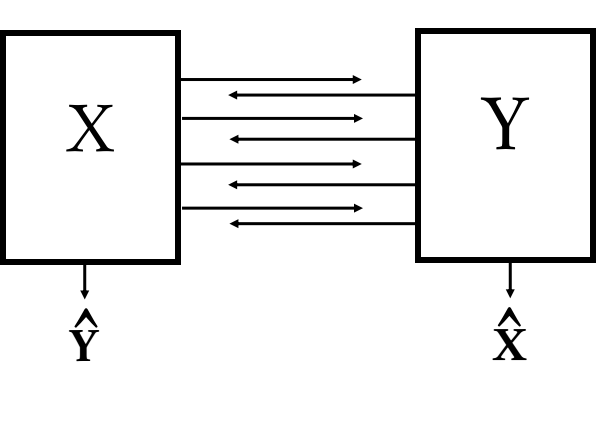
\includegraphics[width=0.4\textwidth]{dataex.png}
  \end{center}
  \caption{The Data-Exchange Problem}
  \label{fig:dataex}
\end{wrapfigure}
A working solution for this problem is r-sync protocol, as described in   \cite{rsync}. The algorithm identifies parts of the source file which are identical to some part of the destination file, and only sends those parts which cannot be matched in this way. Though this protocol is fast and low complexity, it does not exploit the correlation of the data to the best extent possible. In fact, we can view r-sync as an algorithm which uses only one guess, and thus ends up using more communication.\\
In \cite{sw}, David Slepian and Jack Wolf had shown that the optimal solution to this problem is Slepian-Wolf compression. 
\paragraph{Slepian-Wolf Coding Theorem:}states under joint decoding of X and Y a total rate H(X,Y) is sufficient.\\
\begin{wrapfigure}{r}{0.5\textwidth}
  \begin{center}
    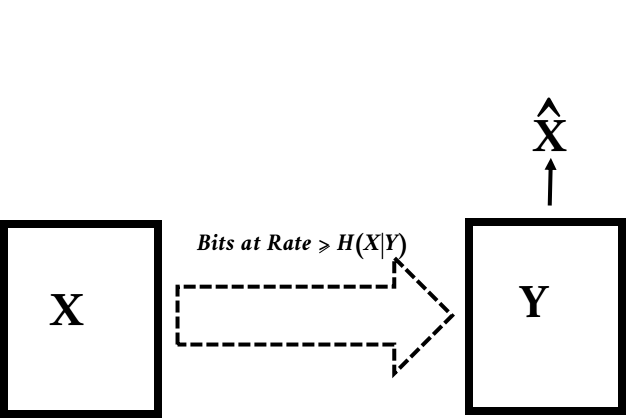
\includegraphics[width=0.4\textwidth]{swcomp.png}
  \end{center}
  \caption{The Slepian-Wolf Compression}
  \label{fig:swcomp}
\end{wrapfigure}
As described in \cite{discus}, consider first the problem where X and Y are correlated discrete-alphabet memoryless sources, we have to compress X losslessly, with Y (side information) being known at the decoder and \emph{not} at the encoder. If Y were known at both ends one can compress X at a theoritical rate of $H(X|Y)$. But if Y were known only at decoder the same can be achieved by just knowing $P_{X|Y}$ at encoder without explicit information of Y, this has been depicted in figure \ref{fig:swcomp}. 
\\\\
A practical implementation of Slepian-Wolf compression faces the following difficulties.
\begin{itemize}
\item Search is over an exponential list in decoding.
\item Knowledge of $P_{X|Y}$ is required.
\end{itemize} 

Using structured channel codes as indicated in \cite{discus}, particularly Polar Codes as shown in \cite{pslep}, alongwith \emph{recursive data exchange protocol}  mentioned in \cite{htsw} for Slepian-Wolf compression eases the aforementioned implementation. 

\subsection{Suggested Approach for Solving The Data-Exchange Problem}\label{suggapp}
In accordance with the above discussion the suggested approach towards solving \emph{The Data-Exchange Problem} may be briefed as follows.
\begin{itemize}
\item{Implement Slepian-Wolf Compression using Polar Codes.}
\item{Achieve universality using \emph{Recursive Data Exchange} protocol (RDE).}
\item{Realise RDE using Rateless Polar Codes with Physical layer Error Detection.}
\end{itemize}

The following sub-sections discuss the artefacts needed for this implementation in brief. Section \ref{propsol}, consolidates and elaborates the proposed scheme. 

\subsection{Interactive Communication for Data Exchange}
The data exchange protocol is based on an interactive version of the Slepian-Wolf protocol where the length of communication is increased in steps until the second party decodes the data of the first. After each transmission second party sends ACK-NACK feedback signal, the protocol stops when ACK is recieved or some pre-decided number of bits ($l_{max}$) have been transmitted \cite{htsw}. Note, this protocol is universal as it does not rely on knowledge of the joint distribution, instead uses an iterative variable length approach to reach rate optimality universally. The decoders suggested in \cite{htsw} are theoritical constructs which use type classes to form a list of guesses for data of other parties and thus has exponential complexity.\\ In \cite{pslep}, Slepian Wolf compression is approached with structered (Polar) codes, in this work we use Rateless Polar Codes to implement RDE with a similar ideology.

\subsection{Brief Introduction to Polar Codes}
\begin{wrapfigure}{r}{0.5\textwidth}
  \begin{center}
    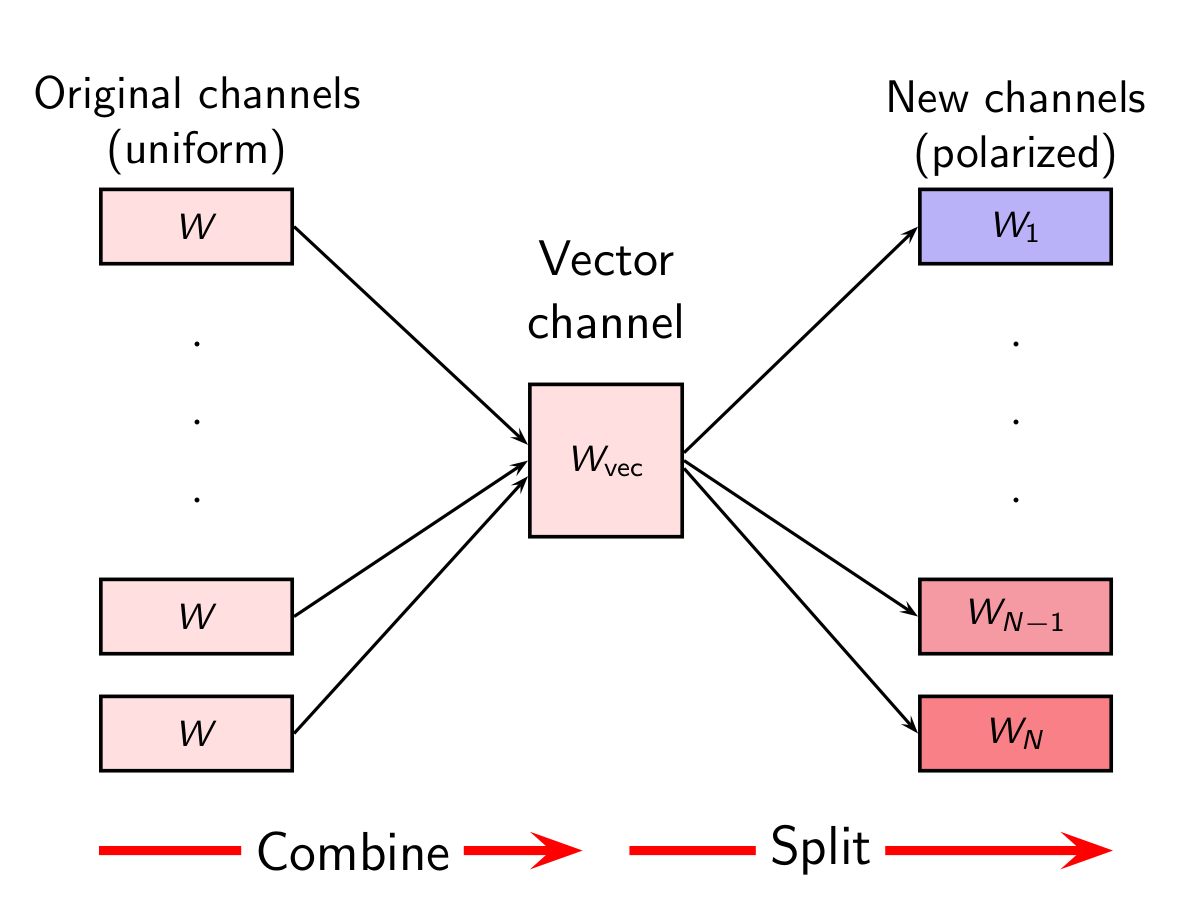
\includegraphics[width=0.4\textwidth]{channelcomb.png}
  \end{center}
  \caption{Channel combining and splitting}
  \label{fig:channelcomb}
\end{wrapfigure}
In 2008, E. Arikan in his paper \cite{arikan} introduced Polar Codes, which provably achieves capacity on symmetric channels. Polar Codes rely on the phenomenon of channel polarization which can be described as follows.
\begin{wrapfigure}{r}{0.5\textwidth}
  \begin{center}
    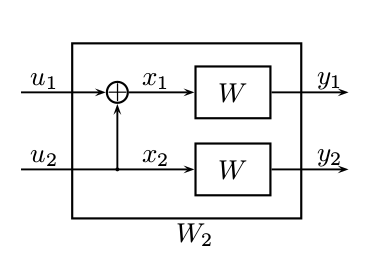
\includegraphics[width=0.4\textwidth]{arikanfly.png}
  \end{center}
  \caption{Arikan transformation butterfly}
  \label{fig:arikanfly}
\end{wrapfigure}
\paragraph{channel polarization}, is an operation by which one manufactures out of N independent copies of a given B-DMC W, a second set of N channels $\{W^{(i)}_N : 1 \leq i \leq N \}$ that show a polarization effect in the sense that, as N becomes large,the symmetric capacity terms $I(W^{(i)}_N )$ tend towards $0$ or $1$,for all but a vanishing fraction of indices i. Hence, Bhattacharya parameter $Z(W^{(i)}_N)$ tend to $1$ or $0$ respectively. The channels with $Z(W^{(i)}_N)=0$ captures the capacity of $W_{vec}$.

This operation consists of a channel combining and a channel splitting phase, as shown in figure \ref{fig:channelcomb}. The channel transformation for two independent channels is shown in \ref{fig:arikanfly}, this is used recursively. \\The encoding process sends data on transformed channels with $Z(W^{(i)}_N)=0$  (\emph{good channels}) and treats the channels with $Z(W^{(i)}_N)=1$ as \emph{bad or frozen}, sending no useful data on them. This scheme of error control coding with polar codes is illustrated in figure \ref{fig:pchscheme}.
\begin{figure}[h]
 \begin{center}
    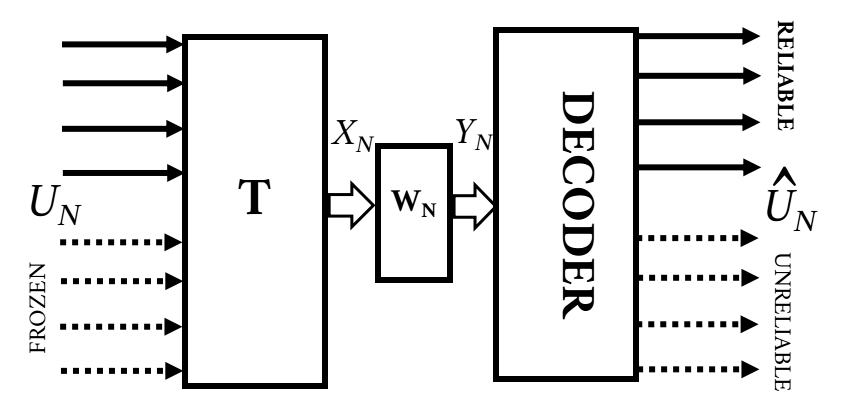
\includegraphics[width=0.6\textwidth]{pchscheme.png}
  \end{center}
  \caption{Polar Coding}
  \label{fig:pchscheme}
\end{figure}\\
In figure \ref{fig:pchscheme}, $U_N$ is a uniform message vector, $T$ is a linear transform equivalent to the butterfly in figure \ref{fig:arikanfly} for a block length of N. $W_N$ is analogous to $W_{vec}$. It is useful to note here that $T=T^{-1}$.
\begin{figure}[h]
  \begin{center}
    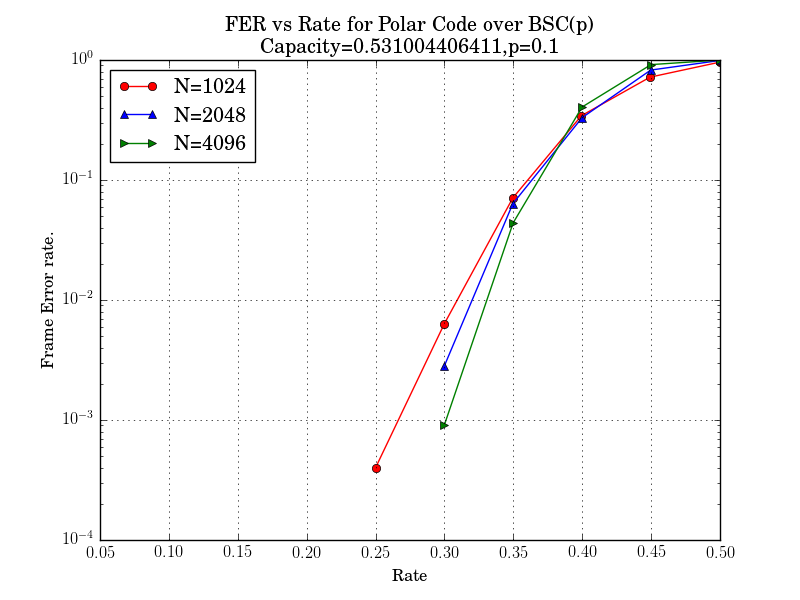
\includegraphics[width=0.6\textwidth]{fer.png}
  \end{center}
  \caption{FER vs Rate for Polar Coding with SC}
  \label{fig:fer}
\end{figure}\\
For our purpose, we shall be using Succesive Cancellation (SC) decoding. Each independent channel will considered as BSC(p). The Polar Code construction indicated in \cite{zhang} has been employed for simplicity. A performance analysis of implementation of the scheme in figure \ref{fig:pchscheme} is presented in figure \ref{fig:fer}    

\subsection{Implementation of SW Compression using Polar Codes}\label{psw}
\begin{figure}[h]
 \begin{center}
    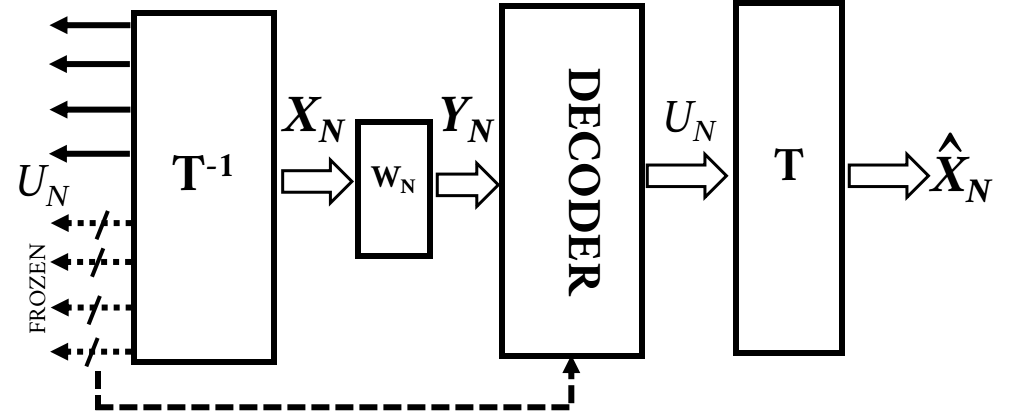
\includegraphics[width=0.6\textwidth]{pswscheme.png}
  \end{center}
  \caption{Polar Coding for SW Compression}
  \label{fig:pswscheme}
\end{figure}
In \cite{discus}, the use of structured codes for Slepian-Wolf compression has been discussed.Further, in \cite{pslep} a specific scheme using Polar Codes has been illustrated, as shown in figure \ref{fig:pswscheme}.
Consider the setting where $X_N$ and $Y_N$ are uniform. $Y_N$ is a corrupted version of $X_N$ by N BSC(p) channel uses. The bits that are to be sent for estimation of $X_N$ from $Y_N$ are the frozen bits in $U_N$. In other words applying $T^{-1}$ to $X_N$ and choosing the bits at frozen positions (the syndrome) essentially describes the compression operation. These bits are communicated error free to the SC-Decoder. Thus $H(X_N)-I(W_N)=H(X_N/Y_N)$ bits are sent. On applying $T$ to the output of SC-decoder the estimate $\hat{X}_N$ is received. It is to be noted here that in general the frozen positions are set to $0$ in channel coding but in Slepian-Wolf compression they are non-zero by the nature of the scheme. Performance analysis of this scheme is presented in figure \ref{fig:swfer}.
\begin{figure}[h]
 \begin{center}
    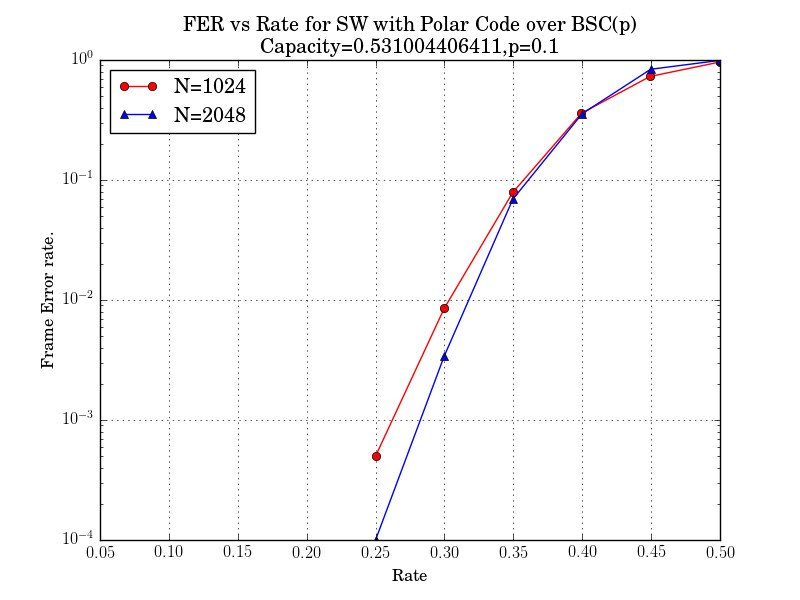
\includegraphics[width=0.6\textwidth]{swfer.png}
  \end{center}
  \caption{FER vs Rate for SW with Polar Code}
  \label{fig:swfer}
\end{figure}\\
Intuitively, a method to generate the syndrome incrementally will lead us to an implementation of RDE. Rateless Polar Codes will be instrumental to accomplish this.

\subsection{Rateless Polar codes}
\paragraph{Rateless code:}A rateless coding scheme transmits incrementally more and more coded bits over an unknown channel until all the information bits are decoded reliably by the receiver. A fixed rate code is designed for a specific channel. In contrast, a rateless code is designed for a set of channels and judged for its performance for the entire set (the compound channel). In general a rateless code design is based on hybrid-ARQ techniques and uses code puncturing. \\For Polar Codes, puncturing is not straightforward. Hybrid-ARQ schemes and puncturing of Polar Codes has been proposed and compared in \cite{harqtav},\cite{harqcheng},and \cite{harqchen}.\\ In \cite{chen}, the authors have proposed a provably capacity achieving rateless coding scheme based on Polar Codes. This scheme is useful for broad class of channels as long as they are ordered by degradation\footnote{using construction methods in \cite{wang},\cite{mondelli} this method can be extended to a broader class of \emph{less noisy} ordered channels}. The scheme stems from the inherent nesting property and degradedness of Polar codes, this makes puncturing a relatively simple affair. 

\subsubsection{Degradedness and Nesting Property}
\begin{wrapfigure}{r}{0.5\textwidth}
  \begin{center}
    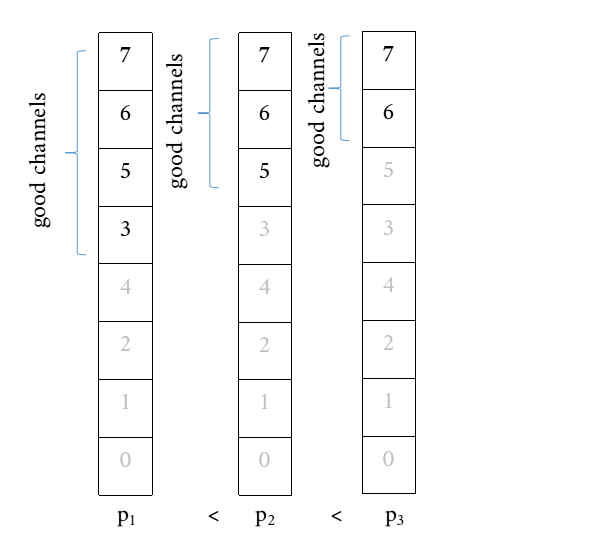
\includegraphics[width=0.5\textwidth]{relorder.png}
  \end{center}
  \caption{Nesting in BSC(p) channels}
  \label{fig:relorder}
\end{wrapfigure}
\paragraph{Degraded channels:}A symmetric binary input channel $W_2$ is said to be degraded with respect to a channel $W_1$ if there exists random variables X,Y,Z such that X\---Y\---Z forms a Markov chain and $W_1=P_{Y|X} , W_2=P_{Z|X}$. By Data Processing Inequality it is evident that the capacity of $W_2$ is lesser than that of $W_1$. This is denoted by $W_2 \preceq W_1$. For example, $BSC(p_1) \preceq BSC(p_2)$ if $p_1 \geq p_2$.
\paragraph{Nesting Property:}Polarization suggests that $W_2 \preceq W_1$ will reflect as lesser number of \emph{good channels} for $W_2$. As the polarization operation preserves degradedness\cite{wang}, the good bit indices of $W_2$ must be a subset of the good bit indices of $W_1$. This is Nesting Property. This leads to a \emph{reliability ordering} of the channels, such that a more reliable channel is always noiseless if a less reliable channel is noiseless regardless of the underlying channel.
\subsubsection{Incremental freezing}\label{if}
Given the reliability ordering, a rateless scheme in \cite{chen} can be described as follows. The initial transmission can be done using a high rate polar code with many information bits and less frozen bits. If this transmission cannot be decoded\footnote{Decodability is checked by CRC in higher layers.} then among the informations bits sent, the ones on comparatively lesser reliable channels are retransmitted. By decoding these bits from future transmissions they effectively become frozen, allowing the rest of the information bits sent on the first transmission to be decoded.  As future transmissions successively freeze more and more bits sent in earlier transmission, this scheme can be called \emph{incremental freezing}.
\begin{figure}[h]
 \begin{center}
    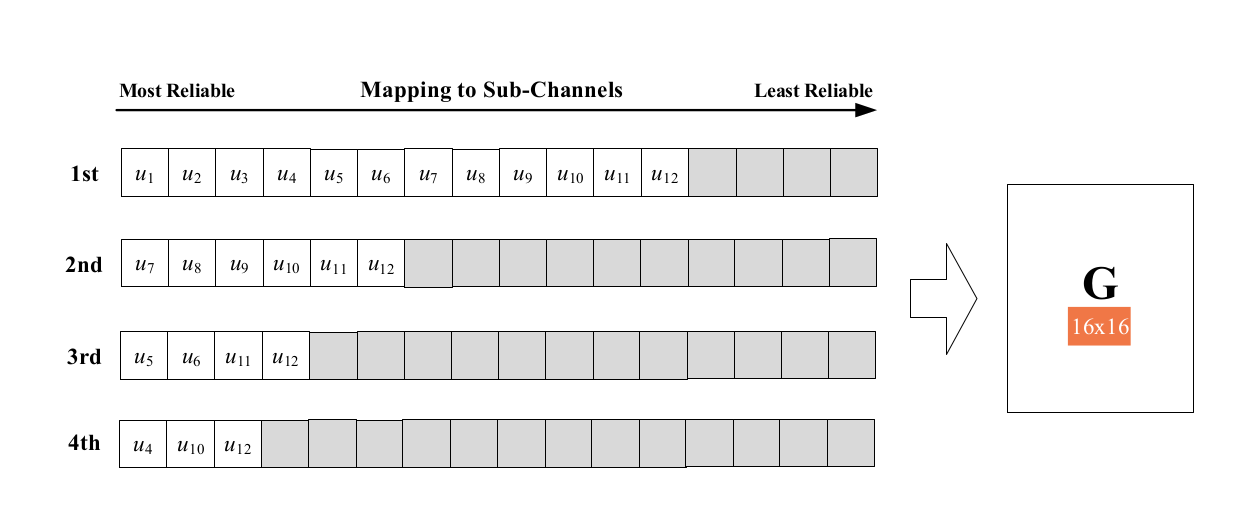
\includegraphics[width=1\textwidth]{if.png}
  \end{center}
  \caption{Incremental freezing for N=16, K=12 and 4 iterations}
  \label{fig:if}
\end{figure}  
\\Figure \ref{fig:if} illustrates the scheme for a set of channels with rates $\{ R=12/16, R_1= R/2,R_2= R/3,R_3= R/4\}$. Here $u_i$ are the message bits. Note that with the $4^{th}$ transmission  $u_4$ to $u_{12}$ has been incrementally frozen. This scheme is capacity achieving in the sense that no rate has been wasted, the final rate achieved is, $$R^*= \frac{12}{16x4}=\frac{3}{16}=R_3 $$. In case the real channel has capacity $ \geq R_3$ the scheme stops at appropriate iteration to achieve that capacity.\\
Though this scheme is not truly rateless as it can achieve only R, R/2, R/3,...rather than a set of arbitrary rates, adding new information bits in future transmissions allow us to rectify this. In similar fashion this can be extended to parallel channels.\\
It is useful to note that a certain number of channels in this scheme is "\emph{always available}" guaranteeing a certain rate in each transmission. A specific application of this will be discussed in section \ref{future}.
\\In \cite{chen}, The performance evaluation of the scheme establishes that $n$ iterations of the scheme is almost equivalent in performance to a $R/n$ fixed rate Polar Code.
\\Adaptation of this scheme for RDE will be indicated in section \ref{propsol}.
\\The following subsections briefly discuss Rateless Polar Coding from the perspective of Hybrid-ARQ.
\subsubsection{H-ARQ for Polar codes}
\paragraph{HYBRID ARQ:}Hybrid automatic repeat request (hybrid ARQ or HARQ) is a combination of high-rate forward error-correcting coding and ARQ error-control. In standard ARQ, redundant bits are added to data to be transmitted using an error-detecting (ED) code such as a cyclic redundancy check (CRC). Receivers detecting a corrupted message will request a new message from the sender. \\In Hybrid ARQ, the original data is encoded with a forward error correction (FEC) code, and the parity bits are either immediately sent along with the message (Type-I) or only transmitted upon request when a receiver detects an erroneous message (Type-II). The retransmission vector is also called the \emph{Redundancy Vector}(RV). \\The ED code may be omitted when a code is used that can perform both forward error correction (FEC) in addition to error detection, such as a Reed-Solomon code or  Turbo Product Code (TPC) \cite{harqmukhtar}.\\The FEC code is chosen to correct an expected subset of all errors that may occur, while the ARQ method is used as a fall-back to correct errors that are uncorrectable using only the redundancy sent in the initial transmission.\\Construction of H-ARQ requires a Rate Compatible Code and a choice of RV (retransmission scheme).
\paragraph{Rate Compatible Codes:}
Given a fixed number of information bits, consider a family of codes $\{C_1,C_2...C_n\}$  with rates $R_1\geq R_2\geq R_3...\geq R_n$, and block lengths $N_1 \leq N_2 \leq ... \leq N_n$.
Then the set is rate compatible if codeword for $C_i$ can be built by removing $N_j-N_i$ bits from codewords of code $C_j$ ,$j\geq i$, \cite{mondelli}. Rate Compatible Codes can be constructed by puncturing low rate codes. 
\\Polar codes for degraded channels is inherently rate compatible due to \emph{reliability ordering} and \emph{nesting}.

\subsubsection*{H-ARQ schemes for Polar Codes}
\begin{wrapfigure}{r}{0.5\textwidth}
  \begin{center}
    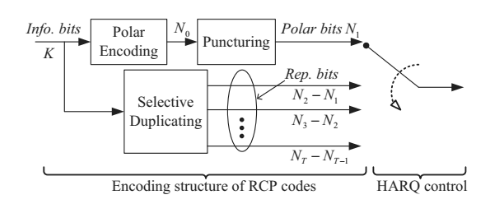
\includegraphics[width=0.5\textwidth]{selrepharq.png}
  \end{center}
  \caption{H-ARQ for Polar Codes with selective repetition}
  \label{fig:selrepharq}
\end{wrapfigure}
In \cite{harqchen}, a H-ARQ scheme for Polar codes based on selective repetition has been studied. The incremental freezing scheme described in \cite{chen} and \cite{mondelli} can be classified as a H-ARQ scheme. In \cite{harqtav} another H-ARQ scheme based on Subset Polar Codes is described along with performance comparison with the other schemes. Here these schemes are discussed in brief. 
\paragraph{H-ARQ for Polar codes with selective repetition:}
As the initial transmission, an information block of K bits is fed into a polar
encoder. The output codeword of $N_0$ bits is punctured into $N_1$
bits and sent over the channel. If the receiver fails to decode
the codeword, an NACK (negative acknowledgement) is sent
to the transmitter through the feedback channel. And then,
$N_2-N_1$ of the information bits are retransmitted. This time,
the receiver tries to perform decoding with all the $N_2$ received
bits. If the decoding is failed again, another $N_3-N_2$ bits
are transmitted. This process continues until the transmitter
receives an ACK (acknowledgement), or a maximum number
of transmissions T is achieved. The scheme has been illustrated in figure  \ref{fig:selrepharq}. The retransmitted bits (RV) are chosen one at a time as the most unreliable of the K bits transmitted, reliability is re-calculated after choosing one bit and the process is iterated.
\paragraph{Incremental freezing:} this scheme is an improvement over the above scheme, it uses the reliability ordering to choose the RV as discussed in \ref{if}.
\paragraph{H-ARQ for Polar codes based on Subset Polar Codes:}
A Subset Polar Code can be created by greedily puncturing a low-rate mother code without re-optimizing the information bits.The scheme uses equivalent subset Polar Codes as RV. In \cite{harqtav}, the author has claimed from simulation results that this scheme performs better among the ones discussed. Nevertheless, we have used incremental freezing for its simplicity.  
\paragraph{Reliability Based H-ARQ:}
It is to be noted that the schemes described above use CRC for checking decodability. Reliability based HARQ technique (RBHARQ) \cite{rbharq}, eliminates the use of CRC by approximating bit and word error probability from likelihood ratios (LLR).  As the magnitude of a log-likelihood value is directly
connected to the error probability of the corresponding
bit, it can be used to determine which bits most
likely caused a word error. The bit error probability for the $k^{th}$ bit can be estimated form LLR ($\tilde{u}_k$) as,
\begin{equation}
P_{b,k}=P(\hat{u_k} \neq u_k) = \frac{1}{1+e^{|\tilde{u}_k|}}
\end{equation}
then word error probability becomes, 
\begin{equation}
P_w=1-e^{log\bar{P}_w}
\end{equation}
where, $$log\bar{P}_w=log\prod_{k=1}^K (1- P_{b,k})$$ 
if the word error probability does not meet the requirements the bits with higher bit error probability may be retransmitted. This retransmission criterion results in increase of throughput, particularly evident in case of short packet lengths.



%----------------------------------------------------------------------------------------
%	PROPOSED SOLUTION
%----------------------------------------------------------------------------------------
\newpage
\section{Proposed implementation of Recursive Data Exchange} \label{propsol}
As indicated in section \ref{intro} and \ref{suggapp}, our approach towards implementation of a solution to \emph{The Data Exchange} using RDE and Polar codes can be summarised as below, 
\begin{itemize}
\item{Use Rateless Polar Codes with Incremental Freezing to implement iterative Slepian-Wolf compression.}
\item{Use a PHY layer error detection as retransmission criterion in Incremantal Freezing.}
\end{itemize}
The following subsections elaborate on the same.




\subsection{Adaptation of Rateless Polar Codes for RDE} 
The RDE, which is essentially an iterative Slepian-Wolf compression, can be constructed using Rateless Polar Code as shown in the example of figure \ref{fig:iswrpc}.
\begin{figure}[h]
 \begin{center}
    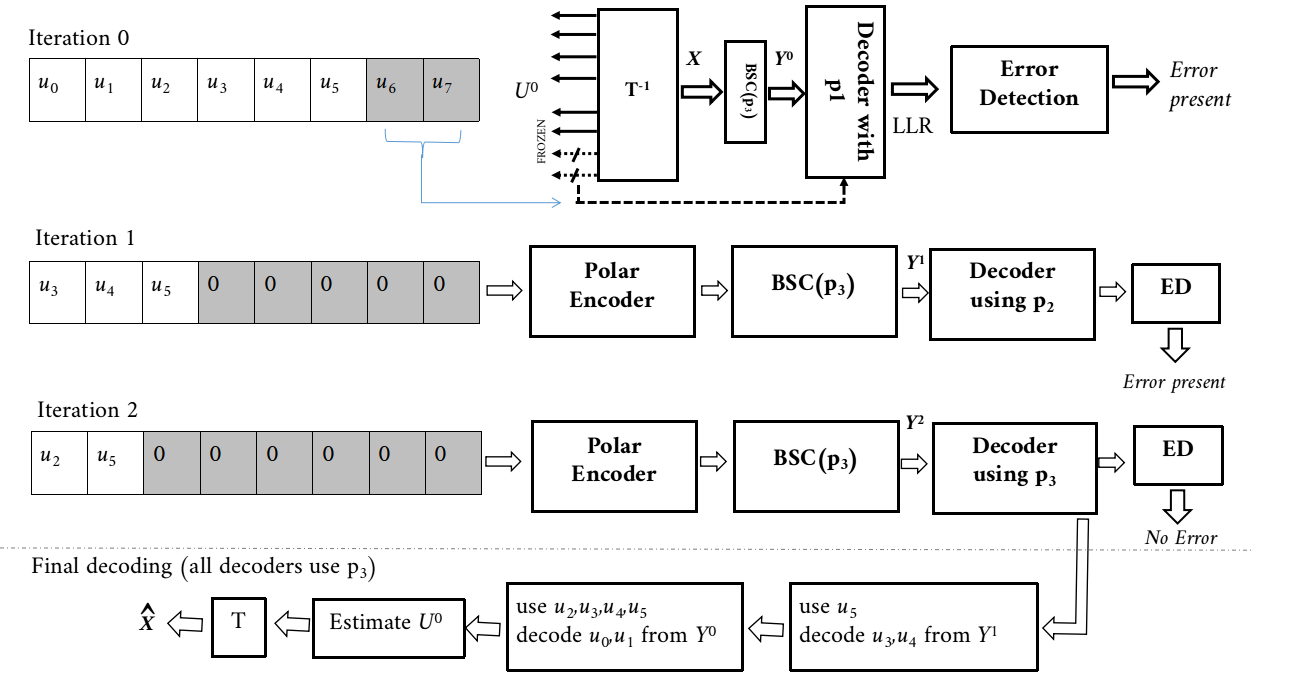
\includegraphics[width=1\textwidth]{iswrpc.png}
  \end{center}
  \caption{Example of Iterative Slepian-Wolf Compression with Incremental Freezing.}
  \label{fig:iswrpc}
\end{figure} 
Here, a compund BSC channel $\mathcal{C}=\{ p_1 \leq p_2 \leq p_3 \leq p_4\}$, is considered, where $p_i$ is the flipover probability of channel $i$. It is assumed that the rates supported by the channels are $\{ R_1=R, R_2= R/2,R_3= R/3,R_4= R/4\}$. The actual channel in the example is BSC($p_3$), henceforth we shall denote this as BSC($p_{channel}$).\\
\paragraph{first Iteration:} In the first iteration, the Slepian-Wolf compression with Polar Coding scheme suggested in figure \ref{fig:pswscheme} is followed. Additionally, the soft outputs(LLRs) generated from the decoder block are passed through an Error Detection (ED) block. In case error is present, receiver replies with a NACK and further iterations are commenced. It is to be noted that the decoder \emph{guesses} the channel to be BSC($p_1$) greedily and computes LLR accordingly. Henceforth we shall denote this as BSC($p_{guess}$). Note, in this iteration the frozen bits are non-zero, and are communicated error-free to receiver.
\paragraph{subsequent iterations:}In the subsequent iterations, the decoder makes greedy guesses about the channel from a subset of the compound channel which does not include previous guesses. In other words, in second iteration $p_{guess}=p_2$, in third $p_{guess}=p_3$. Iterations continue as long as the ED does not declare error-free transmission, which is communicated as ACK by the receiver.\\
The message sent in these iterations consist of information bits which are suspected to be sent unreliably in previous iterations under impression that present $p_{guess}$ is correct, as discussed in section \ref{if} . The frozen bits are set to zero and need not sent to receiver. Transmission is as illustrated in figure \ref{fig:pchscheme}.
\paragraph{Final decoding:}When the ED declares no error the decoder infers that the $p_{channel}=p_{guess}$, let us denote this as $p_{final}$. The decoder now  decodes the bits of penultimate iteration from the channel output of the penultimate iteration using $p_{final}$ and considering the information bits decoded in last iteration as frozen. This continues till all bits are decoded successfully. Finally, with arikan transform X is estimated.
\\\emph{Note, X and Y have there usual meanings as in figure \ref{fig:swcomp}.}  


\subsection{PHY-Layer error Detection} 

A distinct difference between Polar codes for error control and Slepian-Wolf compression using polar codes is that, in the latter the $U_N$ is generated from $X_N$. Hence using a CRC in $U_N$ which can be exploited for error detection and retransmission in Incremental Freezing does not remain feasible.\\This necessitates  

\subsubsection{The Error Detection Test }
\subsection{Proposed Tests}
\subsection{Performance Evaluation}

%--------------------------------------------------------------------------
% CONCLUSION AND FUTURE WORK
%--------------------------------------------------------------------------
\newpage
\section{Conclusion and Future work}\label{future}
proposed scheme
shortpacket
implementation
\begin{definition}
We can redefine $\Omega_i$ as a set of indicator vectors of $A$.Let,
\[
    [\phi_i(A)]_l=\left\{
                \begin{array}{ll}
                  \mathbf{1}_A(l) \text{ if } l < i\\
                  \mathbf{1}_A(l+1) \text{ if } l \ge i.\\
                \end{array}
              \right.
  \]
\begin{align*}
\Omega_i' &\triangleq \{\phi_i(A) \in \{0,1\}^{N-1} : A \in \Omega_i\}\\
\partial_j\Omega_i' &\triangleq \{\phi_i(A) \in \{0,1\}^{N-1}: A \in \partial_j\Omega_i\}.\\& =\{\underline{x} \in \{0,1\}^{N-1} | \mathbb{1}_{\Omega_i}(\underline{x}) \neq  \mathbb{1}_{\Omega_i}(\underline{x}^{(j)})\}
\end{align*}
\label{defn13}
\end{definition}
Here the last equality follows from definition of $\partial_j\Omega_i$.\\
Consider the space $\{0,1\}^M$ ,we can redefine measure $\mu_p$ such that $$\mu_p(\Omega) = \sum_{\underline{x} \in \Omega} p^{|\underline{x}|}(1-p)^{M-|\underline{x}|}, \text{ for }\Omega \subseteq \{0,1\}^M,$$ where the weight $|\underline{x}| = x_1 + x_2 + \ldots + x_M$ is the number of $1$'s in $\underline{x}$. 
\begin{definition}
For a monotone set $\Omega$.The influence of bit $j \in [N]$,is defined by,
$$I_j^{(p)}(\Omega)\triangleq \mu_p(\partial_j\Omega)$$
The total influence in defined by,
$$I^{(p)}\triangleq \sum^N_{j=1}I_j^{(p)}.$$
\label{defn15}
\end{definition}
Using proposition~\ref{propn4}(a) and proposition 7, we have, 
$$h(p)=h_i(p)=\mu_p(\Omega_i')$$
Further,from proposition~\ref{propn4}(b), we get,
$$I_j^{p}(\Omega_i')=\mu_p(\partial_j\Omega_i') = \frac{\partial h_i(\underline{p})}{\partial p_j'}\Bigg|_{\underline{p}=(p,p,\ldots,p)}$$
where $j'$ is given by 
\[
    j'=\left\{
                \begin{array}{ll}
                  j \text{ if } j < i\\
                  j+1 \text{ if } j \ge i.\\
                \end{array}
              \right.
  \]
Since $\mathcal{G}$ is doubly transitive, from propostion~\ref{propn8}, $$I_j^{p}(\Omega_i') = I_k^{p}(\Omega_i') \text{ for all } j,k \in [N-1].$$
Hence,$\Omega_i$ is a \emph{symmetric monotone set.}

The following theorem could be seen as a consequence of the result by Talagrand~\cite{talagrand}.
\begin{theorem}
Let $\Omega$ be a monotone set and suppose that, for all $0 \le p \le 1$, the influences of all bits are equal $I_1^{(p)}(\Omega) = \ldots = I_M^{(p)}(\Omega)$. Then, for any $0 < \epsilon \le 1/2$, $$p_{1-\epsilon} - p_\epsilon \le \frac{2 \log \frac{1-\epsilon}{\epsilon}}{C\log (N-1)},$$ where $p_t = \inf\{p \in [0,1] : \mu_p (\Omega) \ge t\}$ is well defined because $\mu_p(\Omega)$ is strictly increasing in $p$ with $\mu_0(\Omega) = 0$ and $\mu_1(\Omega)=1$.
\label{thm19}
\end{theorem}
\begin{proof}
Using Russo's lemma~\cite{russo}.
\end{proof}
We see that $\Omega_i$ satisfies the conditions of Theorem~\ref{thm19}.
Hence,\\$$\lim_{n \to \infty} (p_{1-\epsilon} - p_\epsilon) = 0.$$
Further , using proposition~\ref{propn11}, we state,\emph{\\$\{\mathcal{C}_n\}$ is capacity achieving on the BEC under bit-MAP decoding.}


%----------------------------------------------------------------------------------------
%	BIBLIOGRAPHY
%----------------------------------------------------------------------------------------
\newpage
\renewcommand{\refname}{\spacedlowsmallcaps{References}} % For modifying the bibliography heading

\bibliographystyle{unsrt}

\bibliography{polarmid.bib} % The file containing the bibliography

%----------------------------------------------------------------------------------------

\end{document}